% !TeX encoding = UTF-8
% !TeX spellcheck = sk_SK
\documentclass[]{tukediphc}
%% -----------------------------------------------------------------
%% tento subor ma kodovanie utf-8
%%
%% na kompilaciu pouzivajte format pdflatex 
%%
%% V pripade problemov kontaktujte Jána Bušu st. (jan.busa@tuke.sk)
%%
%% November 2015
%% -----------------------------------------------------------------
%%
%\usepackage[dvips]{graphicx}
%\DeclareGraphicsExtensions{.eps}
\usepackage[pdftex]{graphicx}
\DeclareGraphicsExtensions{.pdf,.png,.jpg,.mps}
\graphicspath{{figures/}} % priecinok na obrazky
%%


%\usepackage[utf8]{inputenc}  % je v cls-subore
%\usepackage[T1]{fontenc}  % je v cls-subore
\usepackage{lmodern,textcase}
\usepackage[slovak]{babel}
\def\refname{Zoznam použitej literatúry}
\usepackage{latexsym}
\usepackage{dcolumn} % zarovnanie cisiel v tabulke podla des. ciarky
\usepackage{hhline}
\usepackage{amsmath,amsfonts,amssymb}
\usepackage{nicefrac} % pekne zlomky
\usepackage{upgreek} % napr. $\upmu\mathrm{m}$ pre mikrometer ...
\usepackage[final]{showkeys}%color%notref%notcite%final
\usepackage[slovak,noprefix]{nomencl}
\makeglossary % prikaz na vytvorenie suboru .glo


% Pouzit v pripade velkeho poctu subsection v tableofcontents
%\makeatletter
%\renewcommand*\l@subsection{\@dottedtocline{2}{1.5em}{3.5em}}
%\newcommand*\l@subsection{\@dottedtocline{2}{1.5em}{2.3em}}
%\newcommand*\l@subsubsection{\@dottedtocline{3}{3.8em}{3.2em}}
%\makeatother


%\def\thefigure{\Roman{section}.\arabic{figure}}

%\usepackage{parskip}% 'zhusti' polozky obsahu
%% Cislovane citovanie
\usepackage[numbers]{natbib}
%%
%% Citovanie podľa mena autora a roku
%\usepackage{natbib} \citestyle{chicago}
% -----------------------------------------------------------------
%% tlač !!!
\usepackage[pdftex,unicode=true,bookmarksnumbered=true,
bookmarksopen=true,pdfmenubar=true,pdfview=Fit,linktocpage=true,
pageanchor=true,bookmarkstype=toc,pdfpagemode=UseOutlines,
pdfstartpage=1]{hyperref}
\hypersetup{%
baseurl={http://www.tuke.sk/sevcovic},
pdfcreator={pdfcsLaTeX},
pdfkeywords={Optimalizácia, diplomová práca, písanie},
pdftitle={Optimalizácia písania diplomových prác},
pdfauthor={Ján Zelený},
pdfsubject={Bakalárska práca}
} 
%% nehodiace zakomentujte !
\dippraca{Diplomová práca}
%\bakpraca{Bakalárska práca}
%%
\nazov{Optimalizácia písania diplomových prác}
%% ked praca nema 'podnazov' zakomentujte nasledujuci riadok
%% alebo polozku nechajte prazdnu
\podnazov{}
\jazyk{Slovenský}
% anglicky nazov
\title{Diploma writing optimization}
\autor{Aurel Zelenka-Košický}
\veduciprace{doc.~Ing.~Vojtech~Čierny, CSc.}
\konzultanta{Ing.~Matej~Biely, PhD.}
%\konzultantb{RNDr.~Marián~Čierny, DrSc.}
\titul{Bc}
\univerzita{Technická univerzita v~Košiciach}
\fakulta{Fakulta elektrotechniky a informatiky}
\skratkafakulty{FEI}
\katedra{Katedra umelej inteligencie}
\skratkakatedry{KUI}
\odbor{Experimentálna fyzika (pozri zadávací list)}
\specializacia{Fyzika nízkych teplôt}
\abstrakt{Abstrakt je povinnou súčasťou každej práce. Je výstižnou
charakteristikou obsahu dokumentu. Nevyjadruje hodnotiace stanovisko
autora. Má byť taký informatívny, ako to povoľuje podstata práce.
Text abstraktu sa píše ako jeden odstavec. Abstrakt neobsahuje odkazy
na samotný text práce. Mal by mať rozsah 250 až 500 slov. Pri
štylizácii sa používajú celé vety, slovesá v činnom rode a tretej
osobe. Používa sa odborná terminológia, menej zvyčajné termíny,
skratky a~symboly sa pri prvom výskyte v texte definujú.}
\klucoveslova{Optimalizácia, diplomová práca, písanie}
\abstrakte{Text abstraktu v~svetovom jazyku je potrebný pre integráciu
do medzinárodných informačných systémov. Ak nie je možné cudzojazyčnú
verziu abstraktu umiestniť na jednej strane so slovenským abstraktom,
je potrebné umiestniť ju na samostatnú stranu (cudzojazyčný abstrakt
nemožno deliť a~uvádzať na dvoch strabách).}
\keywords{Optimization, diploma, writing}
\datumodovzdania{11.~4.~2016}
\datumobhajoby{15.~6.~2016}
\mesto{Košice}
\pocetstran{\pageref{page:posledna}}
\kategoria{Záverečná práca}

\begin{document}
\renewcommand{\figurename}{Obrázok}	
\renewcommand\theHfigure{\theHsection.\arabic{figure}}
\renewcommand\theHtable{\theHsection.\arabic{table}}
\bibliographystyle{dcu}

\prvastrana

\titulnastrana

%\analytickylist


%\errata % zaciatok erraty
%Ak je potrebné, autor na tomto mieste opraví chyby, ktoré našiel po
%vytlačení práce. Opravy sa uvádzajú takým písmom, akým je napísaná
%práca. Ak zistíme chyby až po vytlačení a zviazaní práce, napíšem
%erráta na samostatný lístok, ktorý vložíme na toto miesto. Najlepšie je
%lístok prilepiť \citep{kat}.
%
%Forma:
%
%%\tabcolsep=10pt
%\begin{table}[!hb]
%	\centering
%	\begin{tabular}{|c|c|c|c|}\hline
%Strana & Riadok & Chybne & Správne \\\hline\hline
%12 & 6 & publikácia & prezentácia \\\hline
%22 & 23 & internet & intranet \\\hline
%& & & \\\hline
%& & & \\\hline
%	\end{tabular}
%\end{table}
%\kerrata % koniec erraty

\abstraktsk % abstrakt v SK 

\abstrakteng % abstrakt v ENG

\kabstrakt % koniec abstraktov, nova strana

% Na tomto mieste bude vložené zadanie diplomovej práce
\zadanieprace

\cestnevyhlasenie
% Niektorí autori metodických príručiek o~záverečných prácach sa
% nazdávajú, že takéto vyhlásenie je zbytočné, nakoľko povinnosť
% vypracovať záverečnú prácu samostatne, vyplýva študentovi zo zákona a
% na autora práce sa vzťahuje autorský zákon.

\podakovanie
Na tomto mieste môže byť vyjadrenie poďakovania napr. vedúcemu
diplomovej práce, resp. konzultantom, za pripomienky a~odbornú pomoc
pri vypracovaní diplomovej práce.

Na tomto mieste môže byť vyjadrenie poďakovania napr. vedúcemu
diplomovej práce, respektíve konzultantom, za pripomienky a~odbornú
pomoc pri vypracovaní diplomovej práce.

Na tomto mieste môže byť vyjadrenie poďakovania napr. vedúcemu
diplomovej práce alebo konzultantom za pripomienky a~odbornú pomoc pri
vypracovaní diplomovej práce.
\kpodakovania

\predhovor
Predhovor je povinnou náležitosťou záverečnej práce, pozri
\citep{gonda}. V~predhovore autor uvedie základné charakteristiky
svojej záverečnej práce a~okolnosti jej vzniku. Vysvetlí dôvody, ktoré
ho viedli k~voľbe témy, cieľ a~účel práce a~stručne informuje
o~hlavných metódach, ktoré pri spracovaní záverečnej práce použil.
\kpredhovoru

\thispagestyle{empty}
\tableofcontents
\newpage

\thispagestyle{empty}

{	\makeatletter
	\renewcommand{\l@figure}{\@dottedtocline{1}{1.5em}{3.5em}}
	\makeatother
	\listoffigures}

%\addcontentsline{toc}{section}{\numberline{}Zoznam obrázkov}
%\listoffigures


\newpage

\thispagestyle{empty}
%\addcontentsline{toc}{section}{\numberline{}Zoznam tabuliek}
\listoftables
\newpage

\thispagestyle{empty}
%\addcontentsline{toc}{section}{\numberline{}Zoznam symbolov a
%skratiek}
\printglossary % vlozenie zoznamu skratiek a symbolov
\newpage

%\addcontentsline{toc}{section}{\numberline{}Slovník termínov}
\slovnikterminov

\begin{description}
	\item[Dizertácia] je rozsiahla vedecká rozprava, v~ktorej sa na
základe vedeckého výskumu a~s~použitím (využitím) bohatého dokladového
materiálu  ako i~vedeckých metód rieši zložitý odborný problém.
	\item[Font] je súbor, obsahujúci predpisy na zobrazenie textu
v~danom písme, napr. na tlačiarni. To čo vidíme je písmo; font je súbor
a~nevidíme ho.
	\item[Kritika] je odborne vyhrotený, prísny pohľad na hodnotenú
vec. Medzi recenziou a kritikou je taký pomer ako medzi diskusiou a
polemikou. Pri kritike treba prísnosť chápať v~tom zmysle, že sa
v~nej okrem iného navrhuje, ako hodnotené dielo skvalitniť.
	\item[Meter (m)] je vzdialenosť, ktorú svetlo vo vákuu prejde
za čas. interval~$\nicefrac{1}{299\,792\,458}$ sekundy.
	\item[Písmom] rozumieme vlastný vzhľad znakov.
	\item[Problém] termín používaný vo všeobecnom zmysle vo vzťahu
k~akejkoľvek duševnej aktivite, ktorá má nejaký rozoznateľný cieľ.
Samotný cieľ nemusí byť v~dohľadne. Problémy možno charakterizovať
tromi rozmermi -- oblasťou, obtiažnosťou a veľkosťou.
	\item[Proces] je postupnosť či rad časovo usporiadaných
udalostí tak, že každá predchádzajúca udalosť sa zúčastňuje na
determinácii nasledujúcej udalosti.
\end{description}

\kslovnikterminov
%
% !TeX encoding = UTF-8
% !TeX spellcheck = sk_SK
% !TeX root=tukedip.tex
\setcounter{page}{1}
\setcounter{equation}{0}
\setcounter{figure}{0}
\setcounter{table}{0}

\section*{Úvod}
\addcontentsline{toc}{section}{\numberline{}Úvod}
V~úvode autor podrobnejšie ako v~predhovore, pritom výstižne a~krátko
charakterizuje stav poznania alebo praxe v~špecifickej oblasti, ktorá
je predmetom záverečnej práce. Autor presnejšie ako v~predhovore
vysvetlí ciele práce, jej zameranie, použité metódy a~stručne objasní
vzťah práce k~iným prácam podobného zamerania. V~úvode netreba
zachádzať hlbšie do teórie. Nie je potrebné podrobne popisovať metódy,
experimentálne výsledky, ani opakovať závery prípadne odporúčania,
pozri~\citep{kat}.
%
% !TeX encoding = UTF-8
% !TeX spellcheck = sk_SK
% !TeX root=tukedip.tex
\section{Formulácia úlohy}
Na písanie textu záverečnej práce sa používajú štýly uvedené v~tejto
šablóne (Nadpis záverečnej práce, Podnadpis záverečnej práce, Text
záverečnej práce [riadkovanie 1.5, Latin Modern %Times New Roman 
12] a~ďalšie podľa
potreby). Text záverečnej práce musí obsahovať kapitolu s~formuláciou
úlohy resp. úloh riešených v~rámci záverečnej práce. V~tejto časti
autor rozvedie spôsob, akým budú riešené úlohy a~tézy formulované
v~zadaní práce. Taktiež uvedie prehľad podmienok riešenia.
%
% !TeX root=tukedip.tex
% !TeX encoding = UTF-8
% !TeX spellcheck = sk_SK
\section{Analýza}

Text záverečnej práce obsahuje kapitolu, v~rámci ktorej autor uvedie
analýzu riešených problémov. Táto kapitola môže byť v~prípade potreby
delená do viacerých podkapitol. Autor v~texte záverečnej práce môže
zvýrazniť kľúčové slová, pričom sa použije príslušný štýl pre kľúčové
slová -- napr. toto je kľúčové slovo. V~texte môžu byť použité obrázky
a~tabuľky podľa nasledujúcich príkladov:

\begin{figure}[!ht]
\centering \unitlength=1mm
\begin{picture}(30,30)(0,0)
\put(0,0){\line(1,0){30}}
\put(0,0){\line(0,1){30}}
\put(30,0){\line(0,1){30}}
\put(0,30){\line(1,0){30}}
\end{picture}
\caption{Toto je štvorec}\label{o:1}
\end{figure}


Obrázok by mal byť podľa možnosti centrovaný. Pri jeho opisovaní
v~texte treba použiť odkazy na obrázok v~tvare Obrázok~\ref{o:1}.

%\tabcolsep=8pt
\begin{table}[!ht]\caption{Prehľad jednotiek}\label{t:1}
\smallskip
\centering
\begin{tabular}{|l|c|} \hline
Názov	& (Jednotka v~sústave SI) \\ \hline
Napätie & $\upmu$V \\ \hline
\end{tabular}
\end{table}
\nomenclature{$\upmu$}{mikro, $10^{-6}$}
\nomenclature{SI}{Syst\`eme International}
\nomenclature{V}{volt, základná jednotka napätia v sústave SI}

Tabuľka by mala byť podľa možnosti centrovaná. Pri jej opisovaní
v~texte treba použiť odkazy na tabuľku v~tvare: pozri
Tabuľku~\ref{t:1}. Na číslovanie obrázkov, resp. tabuliek treba použiť
triedenie. Za slovom {\it Obrázok} nasleduje ako prvé číslo kapitoly
alebo časti, v~ktorej sa obrázok nachádza, potom medzera, pomlčka,
medzera a~poradové číslo ilustrácie v~danej kapitole alebo časti.
Napr.:~Obrázok~\ref{o:1} (čiže: prvý obrázok v~druhej kapitole alebo
časti). V~prípade, ak tabuľka presahuje stranu, je možné použiť balík
\verb+longtable+.

Navrhujeme zaraďovať obrázky v~elektronickej podobe. Napríklad
Obrázok~\ref{o:2}, ktorý opisuje riešenie diferenciálnej rovnice
tlmených oscilácií
%% \def\ud{\mathrm{d}}
\begin{equation}\label{r:1}
\frac{\ud^2y}{\ud t^2}+\frac{\ud y}{\ud t}+y =0, \qquad y(0)=1, \quad
y\,'(0)=15,
\end{equation}
bol vytvorený v~MATLABe a~príkazom \texttt{print tlmosc.eps -f1
-deps2} bol uložený vo formáte Encapsulated Postscript. Na prípadné
použitie pdf\LaTeX{}u sa obrázok konvertuje do formátu PDF, napr.
pomocou programu \texttt{epstopdf}. Zvyčajne sa číslujú vzťahy, na
ktoré sa v~texte odvolávame. Napríklad: vzťahy (\ref{r:1}) definujú
Cauchyho začiatočnú úlohu.


\begin{figure}[ht!]
\centering
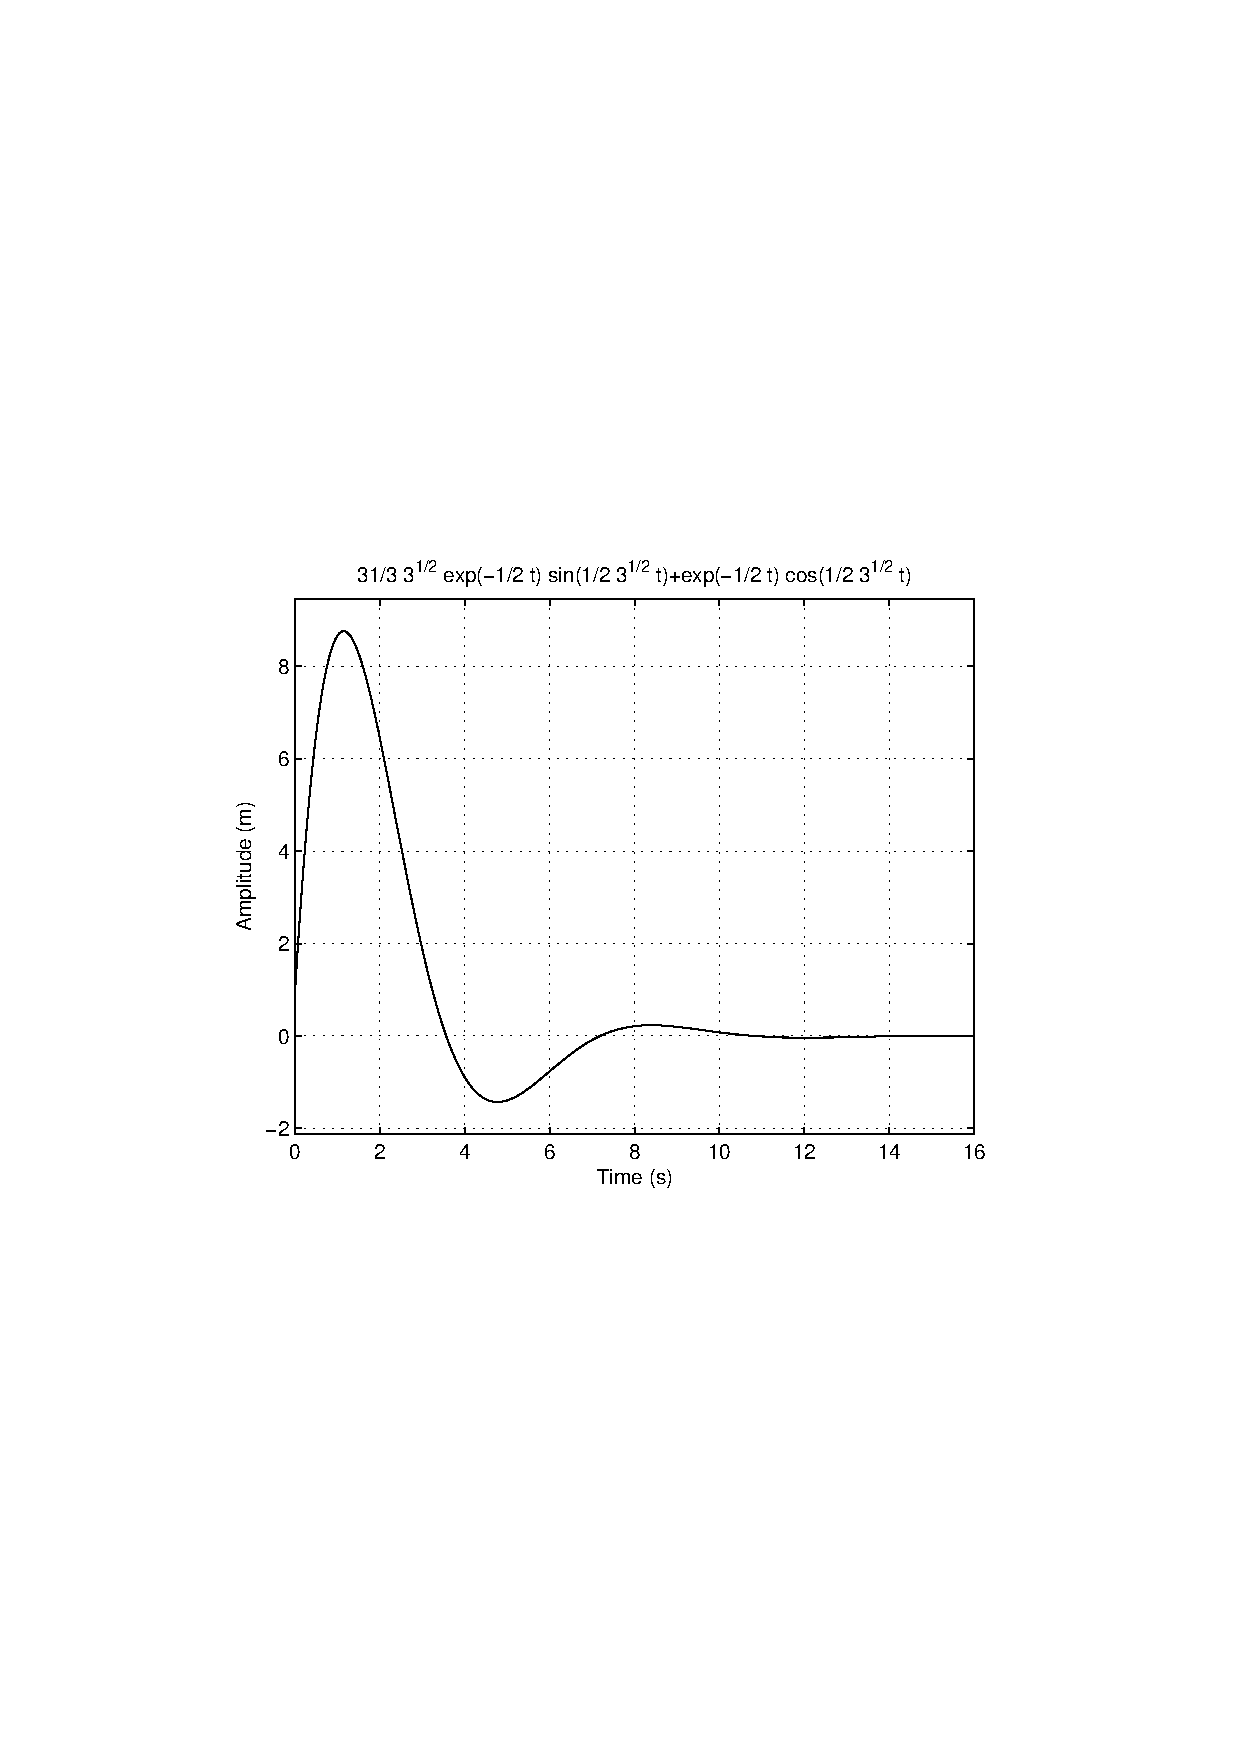
\includegraphics[width=0.7\textwidth]{tlmosc}
\caption{Grafické zobrazenie riešenia rovnice \eqref{r:1}}\label{o:2}
\end{figure}



\subsection{Podkapitola}
Podkapitoly záverečnej práce majú za úlohu členenie textu záverečnej
práce s~cieľom, čo najväčšej prehľadnosti. Kapitol môže byť viacero
a~v~ich názvoch sa používa desatinné číslovanie.
%
% !TeX encoding = UTF-8
% !TeX spellcheck = sk_SK
% !TeX root=tukedip.tex
\section{Jadro práce}

Začnime rovnicou

\begin{equation}\label{r:2}
\frac{\ud^2y}{\ud t^2}+\frac{\ud y}{\ud t}+y =0, \qquad y(0)=1, \quad
y\,'(0)=15.
\end{equation}

Grafický priebeh riešenia tejto rovnice vidíme na Obrázku \ref{o:2}.

\begin{figure}[ht!]
\centering
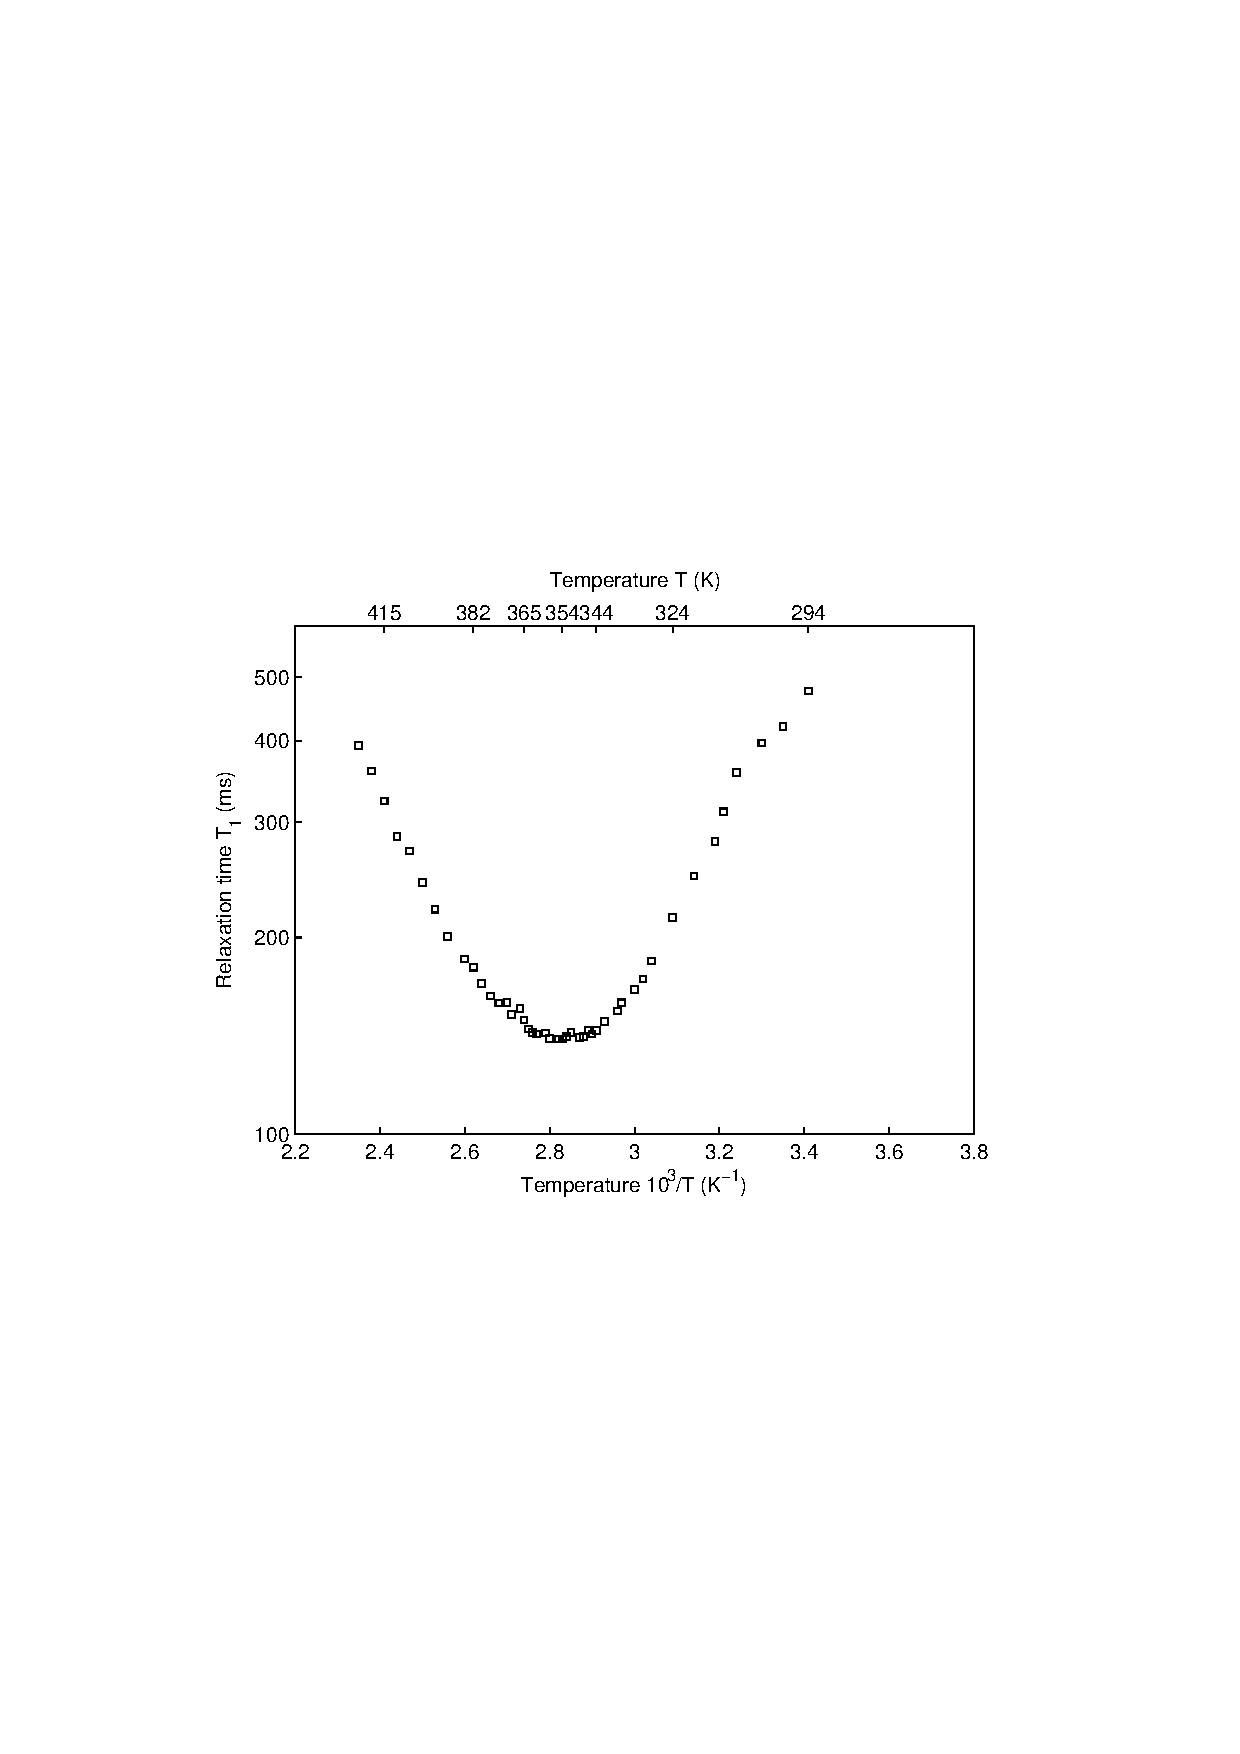
\includegraphics[width=.95\textwidth,angle=0]{relaxcas.pdf}
\caption{Teplotná závislosť spinovo-mriežkového relaxačného
času}\label{o:3}
\end{figure}

%\tabcolsep=3pt % sirka stlpcov
%\renewcommand{\arraystretch}{1.2} % riadkovanie
\begin{table}[ht!]
\centering
\caption{Parametre získané z~meraní spinovo-mriežkových relaxačných
časov $T_1$}\label{t:2}
\medskip
\newcolumntype{d}{D{,}{,}{-1}}
\begin{tabular}{||c||d|d|d|d|d||}
\hhline{|t:==t:==:==:t|}
\multicolumn{1}{||c||}{}&\multicolumn{1}{c|}{PP --
01}&\multicolumn{1}{c|}{PP -- 05}&\multicolumn{1}{c|}{PP --
10}&\multicolumn{1}{c|}{PP -- 16}&\multicolumn{1}{c||}{PP -- 22} \\
\hhline{|:==:==:==:|}
C $\cdot 10^8$~(s$^{-2}$) & 10,1 & 10,0 & 11,0 & 9,2 & 8  \\
\hhline{||-|-|-|-|-|-||}
$\tau_0 \cdot 10^{-14}$~(s) & 2,63 & 1,44 & 0,95 & 2,21 & 10,83  \\
\hhline{||-|-|-|-|-|-||}
$E_{\text a}$~(kJ) & 34,26 & 8,33 & 39,76 & 37,31 & 31,86  \\
\hhline{||-|-|-|-|-|-||}
$T_{\min}$~(K) & 354 & 367 & 367 & 369 & 367  \\
\hhline{||-|-|-|-|-|-||}
$T_{1\min}$~(ms) & 141 & 160 & 157 & 175 & 181  \\
\hhline{||-|-|-|-|-|-||}
$\Delta M_2$~(Gs$^2$) & 5,49 & 5,66 & 5,16 & 5,09 & 5,02  \\
\hhline{|b:==b:==:==:b|}
\end{tabular}
\end{table}


%
\section{Z\'aver (zhodnotenie rie\v{s}enia)}

Táto časť\/ záverečnej práce je povinná. Autor uvedie zhodnotenie
riešenia. Uvedie výhody, nevýhody riešenia,  použitie výsledkov, ďalšie
možnosti a~pod., prípadne načrtne iný spôsob riešenia úloh, resp.
uvedie, prečo postupoval uvedeným spôsobom.
%
% !TeX encoding = UTF-8
% !TeX spellcheck = sk_SK
% !TeX root=tukedip.tex
%%
\begin{thebibliography}{19}
\addcontentsline{toc}{section}{\numberline{}Zoznam použitej literatúry}

\harvarditem{Barančok et al.}{1995}{barancok}
BARANČOK, D. et al. 1995. \emph{The effect of semiconductor surface
treatment on LB film/Si interface.} In:~Physica Status Solidi (a), 
ISSN 0031-8965, 1995, vol. 108, no.~2, \mbox{pp. K~87--90}

\harvarditem{Benčo}{2001}{benco}
BENČO, J. 2001. \emph{Metodológia vedeckého výskumu.} Bratislava~:
IRIS, 2001, ISBN 80\discretionary{-}{-}{-}89018-27-0

\harvarditem{Gonda}{2001}{gonda}
GONDA, V. 2001. \emph{Ako napísať a~úspešne obhájiť diplomovú prácu.}
Bratislava~: Elita, 2001, 3. doplnené a~prepracované vydanie, 120~s.
ISBN 80-8044-075-1

\harvarditem{Jadr. fyz. a~tech.}{1985}{slovnik}
\emph{Jadrová fyzika a~technika: Terminologický výkladový slovník.}
2.~rev.~vyd. Bratislava~: ALFA, 1985. 235~s. ISBN 80-8256-030-5

\harvarditem{Katuščák}{1998}{kat}
KATUŠČÁK, D. 1998. \emph{Ako písať vysokoškolské a~kvalifikačné
práce.} Bratislava~: Stimul, 1998, 2.~doplnené vydanie. 121~s. ISBN
80-85697-82-3

\harvarditem{Lamoš a~Potocký}{1989}{lamos}
LAMOŠ, F. -- POTOCKÝ, R. 1989. \emph{Pravdepodobnosť a~matematická
štatistika.} 1.~vyd. Bratislava~: Alfa, 1989. 344~s. ISBN 80-8046-020-5

\harvarditem{Sýkora a~i.}{1980}{sykora}
SÝKORA, F. a~iní. 1980. \emph{Telesná výchova a~šport.} 1.vyd.
Bratislava~: SPN, 1980. 35~s. ISBN 80-8046-020-5

\harvarditem{Steinerová}{2000}{steinerova}
STEINEROVÁ, J. 2000. \emph{Základy filozofie človeka v~knižničnej
a~informačnej vede.} In:~Kimlička, Š., Knižničná a~informačná veda na
prahu informačnej spoločnosti. Bratislava~: Stimul, 2000. ISBN
80-2274-035-2, s. 327--334

\harvarditem{Šumichrast}{1995}{sumichrast}
ŠUMICHRAST, Ľ. 1995. \emph{On the performance of higher approximations
of radiation boundary conditions for the simulation of wave propagation
in structures of integrated optics.} In:~Photonics '95. Prague~: CTU,
1995, pp. 159--161

\harvarditem{Šumichrast}{1995}{sumichras}
ŠUMICHRAST, Ľ. 1995. \emph{On the performance of higher approximations
	of radiation boundary conditions for the simulation of wave propagation
	in structures of integrated optics.} In:~Photonics '95. Prague~: CTU,
1995, pp. 159--161

\end{thebibliography}
%
\section*{Zoznam pr\'iloh}
\addcontentsline{toc}{section}{\numberline{}Zoznam pr\'iloh}
\thispagestyle{empty}

\begin{description}
	\item[Príloha A] Prílohy
	\item[Príloha B] Bibliografické odkazy
	\item[Príloha C] Vytvorenie zoznamu skratiek a symbolov
	\item[Príloha D] 
\end{description}
%
% !TeX root=tukedip.tex
% !TeX encoding = UTF-8
% !TeX spellcheck = sk_SK
\section*{Príloha A}
\addcontentsline{toc}{section}{\numberline{}Príloha A}
\subsection*{Prílohy}

Táto časť záverečnej práce je povinná a~obsahuje zoznam všetkých
príloh vrátane elektronických nosičov. Názvy príloh v~zozname musia
byť zhodné s~názvami uvedenými na príslušných prílohách. Tlačené
prílohy majú na prvej strane identifikačné údaje -- informácie zhodné
s~titulnou stranou záverečnej práce doplnené o~názov príslušnej
prílohy. Identifikačné údaje sú aj na priložených diskoch alebo
disketách. Ak je médií viac, sú označené aj číselne v~tvare $I/N$, kde
$I$ je poradové číslo a~$N$ je celkový počet daných médií. Zoznam
príloh má nasledujúci tvar:
\begin{description}
\item[Príloha A] CD médium -- záverečná práca v~elektronickej podobe,
prílohy v~elektronickej podobe.
\item[Príloha B] Používateľská príručka
\item[Príloha C] Systémová príručka
\end{description}
Prílohová časť je samostatnou časťou kvalifikačnej práce. Každá
príloha začína na novej strane a je označená samostatným písmenom
(Príloha A, Príloha B, \dots). Číslovanie strán príloh nadväzuje na
číslovanie strán v~hlavnom texte. Pri každej prílohe sa má uviesť
prameň, z~ktorého sme príslušný materiál získali.
%
% !TeX root=tukedip.tex
% !TeX encoding = UTF-8
% !TeX spellcheck = sk_SK
\section*{Príloha B}
\addcontentsline{toc}{section}{\numberline{}Príloha B}
\subsection*{Bibliografické odkazy}

Táto časť záverečnej práce je povinná. V~zozname použitej literatúry
sa uvádzajú odkazy podľa normy STN~ISO~690--2 (01 0197) (Informácie
a~dokumentácia. Bibliografické citácie. Časť 2: Elektronické
dokumenty alebo ich časti, dátum vydania 1.~12.~2001, ICS:~01.140.20).
Odkazy sa môžu týkať knižných, časopiseckých a~iných zdrojov
informácií (zborníky z~konferencií, patentové dokumenty, normy,
odporúčania, kvalifikačné práce, osobná korešpondencia a~rukopisy,
odkazy cez sprostredkujúci zdroj, elektronické publikácie), ktoré boli
v~záverečnej práci použité.

Forma citácií sa zabezpečuje niektorou z~metód, opísaných v~norme
STN~ISO~690, 1998, s.~21. Podrobnejšie informácie nájdete na stránke
\texttt{http://www.tuke.sk/anta/} v~záložke {\small\sf Výsledky
práce/Prehľad normy pre publikovanie STN~ISO~690 a~STN~ISO~690-2}.

Existujú dva hlavné spôsoby citovania v~texte.

\begin{itemize}
\item Citovanie podľa mena a~dátumu.
\item Citovanie podľa odkazového čísla.
\end{itemize}

\emph{Preferovanou metódou citovania} v~texte vysokoškolskej
a~kvalifikačnej práce je podľa normy ISO~7144 citovanie podľa mena
a~dátumu \citep{kat,gonda}. V~tomto prípade sa zoznam použitej
literatúry upraví tak, že za meno sa pridá rok vydania. Na uľahčenie
vyhľadávania citácií sa zoznam vytvára v~abecednom poradí autorov.

\medskip

Príklad:
\dots podľa \citep{steinerova} je táto metóda dostatočne rozpracovaná
na to, aby mohla byť všeobecne používaná v~\dots

\medskip

Druhý spôsob uvedenia odkazu na použitú literatúru je uvedenie len
čísla tohto zdroja v~hranatých zátvorkách bez mena autora (autorov)
najčastejšie na konci príslušnej vety alebo odstavca.

\medskip

Príklad:
\dots podľa [13] je táto metóda dostatočne rozpracovaná na to, aby
mohla byť všeobecne používaná v~\dots ako je uvedené v~[14].

\medskip

Citácie sú spojené s~bibliografickým odkazom poradovým číslom v~tvare
indexu alebo čísla v~hranatých zátvorkách. Odkazy v~zozname na konci
práce budú usporiadané podľa týchto poradových čísel. Viacero citácií
toho istého diela bude mať rovnaké číslo. Odporúča sa usporiadať
jednotlivé položky v~poradí citovania alebo podľa abecedy.

\medskip
\noindent
Rôzne spôsoby odkazov je možné dosiahnuť zmenou voľby v~balíku
\verb+natbib+:

\noindent
\verb+% Citovanie podla mena autora a roku+\\
\verb+\usepackage[]{natbib}\citestyle{chicago}+\\
\verb+% Možnosť rôznych štýlov citácií. Príklady sú uvedené+\\
\verb+% v preambule súboru natbib.sty.+\\
\verb+% Napr. štýly chicago, egs, pass, anngeo, nlinproc produkujú+\\
\verb+% odkaz v tvare (Jones, 1961; Baker, 1952). V prípade, keď+\\
\verb+% neuvedieme štýl citácie (vynecháme \citestyle{}) v "options"+\\
\verb+% balíka natbib zapíšeme voľbu "colon".+

\medskip
\noindent
Keď zapneme voľbu \verb+numbers+, prepneme sa do režimu citovania
podľa odkazového čísla.

\noindent
\verb+% Metoda ciselnych citacii+\\
\verb+\usepackage[numbers]{natbib}+

\bigskip

Pri zápise odkazov sa používajú nasledujúce pravidlá:

V~odkaze na knižnú publikáciu (pozri príklad zoznamov na konci tejto
časti):
\begin{itemize}
\item Uvádzame jedno, dve alebo tri prvé mená oddelené pomlčkou,
ostatné vynecháme a~namiesto nich napíšeme skratku et al. alebo a~i.
\item Podnázov sa môže zapísať vtedy, ak to uľahčí identifikáciu
dokumentu. Od názvu sa oddeľuje dvojbodkou a~medzerou.
\item Dlhý názov sa môže skrátiť v~prípade, ak sa tým nestratí
podstatná informácia. Nikdy sa neskracuje začiatok názvu. Všetky
vynechávky treba označiť znamienkami vypustenia  \uv{\dots}
\end{itemize}

Pri využívaní informácií z~elektronických dokumentov  treba
dodržiavať tieto zásady:
\begin{itemize}
\item  uprednostňujeme autorizované súbory solídnych služieb
a~systémov,
\item zaznamenáme dostatok informácií o~súbore tak, aby ho bolo opäť
možné vyhľadať,
\item urobíme si kópiu použitého prameňa v~elektronickej alebo
papierovej forme,
\item za verifikovateľnosť informácií zodpovedá autor, ktorý sa na
ne odvoláva.
\end{itemize}

Pre zápis elektronických dokumentov platia tie isté pravidlá, ako pre
zápis \uv{klasických}. Navyše treba uviesť tieto údaje:
\begin{itemize}
\item  druh nosiča  [online], [CD-ROM], [disketa], [magnetická páska]
\item dátum citovania  (len pre online dokumenty)
\item dostupnosť  (len pre online dokumenty)
\end{itemize}

Poradie prvkov odkazu je nasledovné:
Autor. Názov. In Názov primárneho zdroja: Podnázov. [Druh  nosiča].
Editor. Vydanie alebo verzia. Miesto vydania : Vydavateľ, dátum
vydania. [Dátum citovania]. Poznámky.  Dostupnosť. ISBN alebo ISSN.
%
% !TeX encoding = UTF-8
% !TeX spellcheck = sk_SK
% !TeX root=tukedip.tex
\section*{Príloha C}
\addcontentsline{toc}{section}{\numberline{}Príloha C}
\subsection*{Vytvorenie zoznamu skratiek a symbolov}

Ak sú v~práci skratky a symboly, vytvára sa \emph{Zoznam skratiek
a~symbolov} (a~ich dešifrovanie). V~prostredí \LaTeX{}u sa takýto
zoznam
ľahko vytvorí pomocou balíka \verb+nomencl+. Postup je nasledovný:
\begin{enumerate}
\item Do preambuly zapíšeme nasledujúce príkazy\\
\verb+\usepackage[slovak,noprefix]{nomencl}+\\ \verb+\makeglossary+
\item  V~mieste, kde má byť vložený zoznam zapíšeme príkaz\\
\verb+\printglossary+
\item V miestach, kde sa vyskytujú skratky a symboly ich definíciu
zavedieme, napr. ako     	v~našom texte, príkazmi\\
\verb+\nomenclature{$\upmu$}{mikro, $10^{-6}$}+\\
\verb+\nomenclature{V}{volt, základná jednotka napätia v sústave SI}+\\
a dokument \uv{pre\LaTeX{}ujeme}.
\item Z~príkazového riadka spustíme program \verb+makeindex+
s~prepínačmi podľa použitého operačného systému, napr.~v~OS~GNU/Linux
s~distribúciou Ubuntu~$10.04$ a~verziou \verb+texlive 2009-7+
napíšeme:\\
\verb*+makeindex tukedip.glo -s nomencl.ist -o tukedip.gls+\\
~v~OS~Win\,XP s~verziou \verb+TeXLive 2010+
napíšeme:\\
\verb*+makeindex -o tukedip.gls -s nomencl.ist tukedip.glo+

\item Po opätovnom \uv{pre\LaTeX{}ovaní} dokumentu sa na
požadované
miesto vloží \emph{Zoznam skratiek a symbolov}.
\end{enumerate}

%
% zivotopis autora
\newpage
\phantomsection
\protect\label{page:posledna}
\curriculumvitae
Táto časť je nepovinná. Autor tu môže uviesť svoje biografické
údaje, údaje o~záujmoch, účasti na~projektoch, účasti na~súťažiach,
získané ocenenia, zahraničné pobyty na~praxi, domácu prax, publikácie
a~pod.
\kcurriculumvitae

\end{document}
%%